\documentclass[11pt, a4paper]{article}

% Fonts and Encoding
\usepackage[utf8]{inputenc}
\usepackage[T1]{fontenc}
\usepackage{lmodern}

% Math and Symbols
\usepackage{amsmath, amssymb, amsthm, amsfonts, mathrsfs, mathtools}

% Layout and Geometry
\usepackage{geometry}
\geometry{a4paper, margin=1in}

% Formatting and Graphics
\usepackage{graphicx, xcolor, enumitem, booktabs, array, tabularx}

% TikZ for Illustrations
\usepackage{tikz}
\usetikzlibrary{arrows.meta, positioning, shapes.geometric, calc, backgrounds, matrix}

% Clickable Links and TOC
\usepackage{hyperref}
\hypersetup{
    colorlinks=true,
    linkcolor=blue,
    filecolor=magenta,      
    urlcolor=cyan,
    pdftitle={Advanced Mathematics: Equivalence Relations},
}

% Theorem Environments
\newtheorem{theorem}{Theorem}[section]
\newtheorem{lemma}[theorem]{Lemma}
\newtheorem{proposition}[theorem]{Proposition}
\newtheorem{corollary}[theorem]{Corollary}
\theoremstyle{definition}
\newtheorem{definition}{Definition}[section]
\newtheorem{axiom}{Axiom}[section]
\newtheorem{example}{Example}[section]
\theoremstyle{remark}
\newtheorem{remark}{Remark}[section]

% Custom Commands (Enforced standard notation)
\newcommand{\R}{\mathbb{R}}
\newcommand{\N}{\mathbb{N}}
\newcommand{\Z}{\mathbb{Z}}
\newcommand{\Q}{\mathbb{Q}}
\newcommand{\E}{\mathbb{E}}
\newcommand{\Prob}{\mathbb{P}}
\newcommand{\F}{\mathcal{F}}

\begin{document}

\title{\textbf{Advanced Abstract Mathematics: Equivalence Relations and Partitions}}
\author{Tashfeen Omran}
\date{\today}
\maketitle

\tableofcontents
\newpage

\section{Comprehensive Introduction, Context, and Prerequisites}

\subsection{Core Concepts and Axioms}
In the foundational architecture of abstract mathematics, an \textbf{Equivalence Relation} is a formal mechanism used to generalize the concept of equality. While strict equality ($=$) demands that two objects be identical in every conceivable aspect, an equivalence relation allows us to declare two distinct objects as "equivalent" provided they share a specific, defining characteristic. 

Let $A$ be a non-empty set. A relation $R$ on $A$ is a subset of the Cartesian product $A \times A$. We write $a R b$ to denote $(a, b) \in R$. For $R$ to be classified as an equivalence relation, it must satisfy three axiomatic properties:
\begin{enumerate}
    \item \textbf{Reflexivity:} For every $a \in A$, $a R a$. (Every element is related to itself).
    \item \textbf{Symmetry:} For every $a, b \in A$, if $a R b$, then $b R a$. (The relation is bidirectional).
    \item \textbf{Transitivity:} For every $a, b, c \in A$, if $a R b$ and $b R c$, then $a R c$. (The relation chains logically).
\end{enumerate}

When $R$ is an equivalence relation on $A$, it naturally fragments $A$ into disjoint subsets called \textbf{Equivalence Classes}. The equivalence class of an element $a \in A$, denoted $[a]$, is defined as:
\[ [a] = \{ x \in A : x R a \} \]

\subsection{Intuition and Set-Theoretic Foundations}
Intuitively, an equivalence relation acts as a mathematical "sorting hat." Imagine a room full of people (the set $A$). If we define a relation $R$ such that $x R y$ if "$x$ and $y$ were born in the same month," this relation is reflexive (you share a birth month with yourself), symmetric (if you share with Bob, Bob shares with you), and transitive (if you share with Bob, and Bob with Alice, you share with Alice). 

Set-theoretically, this sorting process creates a \textbf{Partition} of the set $A$. A partition is a collection of non-empty, pairwise disjoint subsets of $A$ whose union is exactly $A$. The profound beauty of equivalence relations lies in the \textit{Fundamental Theorem of Equivalence Relations}: Every equivalence relation on a set produces a unique partition of that set, and conversely, every partition of a set defines a unique equivalence relation.

\subsection{Historical Context and Motivation}
The formalization of equivalence relations emerged during the 19th century as mathematicians sought to rigorously define number systems and algebraic structures. Carl Friedrich Gauss's introduction of modular arithmetic in his 1801 masterpiece \textit{Disquisitiones Arithmeticae} was a watershed moment. Gauss realized that integers could be grouped into classes based on their remainders when divided by a prime number, effectively treating infinite sets of numbers as single algebraic entities. This necessitated a formal logical framework to handle "equality up to a certain condition," birthing the modern equivalence relation.

\subsection{Key Theorems and Formulas}
\begin{theorem}[Equivalence Class Equality]
Let $R$ be an equivalence relation on a set $A$, and let $a, b \in A$. Then $[a] = [b]$ if and only if $a R b$.
\end{theorem}
\begin{theorem}[The Partition Theorem]
Let $R$ be an equivalence relation on a non-empty set $A$. The set of distinct equivalence classes resulting from $R$ forms a partition of $A$.
\end{theorem}

\subsection{Prerequisites}
To master this chapter, the reader must possess:
\begin{itemize}
    \item \textbf{Set Theory:} Fluency in Cartesian products, subsets, unions, and intersections.
    \item \textbf{Logic:} Understanding of conditional statements ($\implies$), biconditionals ($\iff$), and quantifiers ($\forall, \exists$).
    \item \textbf{Proof Techniques:} Proficiency in Direct Proofs, Proof by Contradiction, and algebraic manipulation (especially concerning divisibility and parity).
\end{itemize}

\newpage

\section{Detailed Homework Solutions (Rigorous Proofs \& Computations)}

This section provides rigorous, step-by-step solutions to the exercises from Section 9.3 (Problems 9.24 through 9.35).

\subsection{Problem 9.24}
\textbf{Statement:} Let $R$ be an equivalence relation on $A = \{a, b, c, d, e, f, g\}$ such that $a R c$, $c R d$, $d R g$, and $b R f$. If there are three distinct equivalence classes resulting from $R$, determine these equivalence classes and determine all elements of $R$.

\textbf{Solution:}
\textit{Proof Technique: Constructive Deduction via Equivalence Properties.}
1. By the transitive and symmetric properties of equivalence relations, elements related to each other belong to the same equivalence class.
2. We are given $a R c$, $c R d$, and $d R g$. 
   - Since $a R c$, we have $[a] = [c]$.
   - Since $c R d$, we have $[c] = [d]$.
   - Since $d R g$, we have $[d] = [g]$.
   - Therefore, $\{a, c, d, g\} \subseteq [a]$.
3. We are given $b R f$.
   - Therefore, $[b] = [f]$, meaning $\{b, f\} \subseteq [b]$.
4. The set $A$ contains $7$ elements. We have accounted for $a, b, c, d, f, g$. The only remaining element is $e$.
5. We are given that there are exactly three distinct equivalence classes. The classes we have partially constructed are $[a]$ and $[b]$. If $e$ belonged to $[a]$ or $[b]$, there would only be two distinct classes (or fewer). To satisfy the condition of exactly three distinct classes, $e$ must form its own equivalence class.
6. Thus, the three distinct equivalence classes are:
   \[ C_1 = \{a, c, d, g\}, \quad C_2 = \{b, f\}, \quad C_3 = \{e\} \]
7. The relation $R$ is the union of the Cartesian products of each equivalence class with itself, because every element in a class is related to every other element in that same class, and to nothing else.
   \[ R = (C_1 \times C_1) \cup (C_2 \times C_2) \cup (C_3 \times C_3) \]
8. Enumerating the elements:
   - $C_1 \times C_1$ yields $4 \times 4 = 16$ pairs: $(a,a), (a,c), (a,d), (a,g), (c,a), (c,c), (c,d), (c,g), (d,a), (d,c), (d,d), (d,g), (g,a), (g,c), (g,d), (g,g)$.
   - $C_2 \times C_2$ yields $2 \times 2 = 4$ pairs: $(b,b), (b,f), (f,b), (f,f)$.
   - $C_3 \times C_3$ yields $1 \times 1 = 1$ pair: $(e,e)$.
   
\textbf{Conclusion:} The equivalence classes are $\{a, c, d, g\}$, $\{b, f\}$, and $\{e\}$. The relation $R$ contains the 21 ordered pairs listed above. $\blacksquare$

\subsection{Problem 9.25}
\textbf{Statement:} Let $A = \{1, 2, 3, 4, 5, 6\}$. The relation $R = \{(1,1), (1,5), (2,2), (2,3), (2,6), (3,2), (3,3), (3,6), (4,4), (5,1), (5,5), (6,2), (6,3), (6,6)\}$ is an equivalence relation on $A$. Determine the distinct equivalence classes.

\textbf{Solution:}
\textit{Proof Technique: Direct Computation of Equivalence Classes.}
1. The equivalence class of an element $x \in A$ is $[x] = \{ y \in A : (y, x) \in R \}$.
2. Let us evaluate the class for $1$:
   - Looking at $R$, the pairs ending in $1$ are $(1,1)$ and $(5,1)$. Thus, $[1] = \{1, 5\}$.
3. Let us evaluate the class for $2$:
   - The pairs ending in $2$ are $(2,2), (3,2), (6,2)$. Thus, $[2] = \{2, 3, 6\}$.
4. Let us evaluate the class for $4$:
   - The only pair ending in $4$ is $(4,4)$. Thus, $[4] = \{4\}$.
5. We check if the union of these classes covers $A$: $\{1, 5\} \cup \{2, 3, 6\} \cup \{4\} = \{1, 2, 3, 4, 5, 6\} = A$. Since equivalence classes partition the set, we have found all distinct classes.

\textbf{Conclusion:} The distinct equivalence classes are $\{1, 5\}$, $\{2, 3, 6\}$, and $\{4\}$. $\blacksquare$

\subsection{Problem 9.26}
\textbf{Statement:} Let $A = \{1, 2, 3, 4, 5, 6\}$. The distinct equivalence classes resulting from an equivalence relation $R$ on $A$ are $\{1, 4, 5\}$, $\{2, 6\}$, and $\{3\}$. What is $R$?

\textbf{Solution:}
\textit{Proof Technique: Constructive Definition of $R$ from a Partition.}
1. By the Partition Theorem, if we are given the equivalence classes, the relation $R$ consists of all pairs $(x, y)$ such that $x$ and $y$ belong to the same equivalence class.
2. Let $C_1 = \{1, 4, 5\}$, $C_2 = \{2, 6\}$, and $C_3 = \{3\}$.
3. $R = (C_1 \times C_1) \cup (C_2 \times C_2) \cup (C_3 \times C_3)$.
4. We compute each Cartesian product:
   - $C_1 \times C_1 = \{(1,1), (1,4), (1,5), (4,1), (4,4), (4,5), (5,1), (5,4), (5,5)\}$
   - $C_2 \times C_2 = \{(2,2), (2,6), (6,2), (6,6)\}$
   - $C_3 \times C_3 = \{(3,3)\}$
5. Taking the union of these sets gives the complete relation $R$.

\textbf{Conclusion:} $R = \{(1,1), (1,4), (1,5), (4,1), (4,4), (4,5), (5,1), (5,4), (5,5), (2,2), (2,6), (6,2), (6,6), (3,3)\}$. $\blacksquare$

\subsection{Problem 9.27}
\textbf{Statement:} Let $R$ be a relation defined on $\Z$ by $a R b$ if $a^3 = b^3$. Show that $R$ is an equivalence relation on $\Z$ and determine the distinct equivalence classes.

\textbf{Solution:}
\textit{Proof Technique: Direct Proof of Equivalence Properties.}
1. \textbf{Reflexivity:} Let $a \in \Z$. Since equality is reflexive, $a^3 = a^3$. Therefore, $a R a$. $R$ is reflexive.
2. \textbf{Symmetry:} Let $a, b \in \Z$ and assume $a R b$. By definition, $a^3 = b^3$. By the symmetry of equality, $b^3 = a^3$. Therefore, $b R a$. $R$ is symmetric.
3. \textbf{Transitivity:} Let $a, b, c \in \Z$ and assume $a R b$ and $b R c$. This means $a^3 = b^3$ and $b^3 = c^3$. By the transitivity of equality, $a^3 = c^3$. Therefore, $a R c$. $R$ is transitive.
4. Since $R$ is reflexive, symmetric, and transitive, it is an equivalence relation.
5. \textbf{Equivalence Classes:} We must find all $b \in \Z$ such that $b R a$, which means $b^3 = a^3$. In the set of real numbers (and thus in $\Z$), the function $f(x) = x^3$ is strictly monotonically increasing and therefore injective (one-to-one). Thus, $b^3 = a^3 \implies b = a$.
6. Therefore, the equivalence class of any integer $a$ is simply $[a] = \{a\}$.

\textbf{Conclusion:} $R$ is an equivalence relation, and the distinct equivalence classes are the singleton sets $\{a\}$ for every $a \in \Z$. $\blacksquare$

\subsection{Problem 9.28}
\textbf{Statement:} 
(a) Let $R$ be the relation defined on $\Z$ by $a R b$ if $a + b$ is even. Show that $R$ is an equivalence relation and determine the distinct equivalence classes.
(b) Suppose that "even" is replaced by "odd" in (a). Which of the properties reflexive, symmetric, and transitive does $R$ possess?

\textbf{Solution:}
\textit{Proof Technique: Direct Proof using Parity Arguments.}

\textbf{Part (a):}
1. \textbf{Reflexivity:} Let $a \in \Z$. Then $a + a = 2a$. Since $2a$ is an integer multiple of 2, $a + a$ is even. Thus, $a R a$.
2. \textbf{Symmetry:} Let $a, b \in \Z$ and assume $a R b$. Then $a + b$ is even. Since addition is commutative, $b + a = a + b$, so $b + a$ is also even. Thus, $b R a$.
3. \textbf{Transitivity:} Let $a, b, c \in \Z$ and assume $a R b$ and $b R c$. Then $a + b = 2k$ and $b + c = 2j$ for some $k, j \in \Z$. Adding these equations yields $(a + b) + (b + c) = 2k + 2j$, which simplifies to $a + c + 2b = 2(k + j)$. Rearranging gives $a + c = 2(k + j - b)$. Since $k + j - b \in \Z$, $a + c$ is even. Thus, $a R c$.
4. \textbf{Equivalence Classes:} $a + b$ is even if and only if $a$ and $b$ have the same parity (both even or both odd). Thus, there are exactly two equivalence classes: the set of all even integers, and the set of all odd integers.

\textbf{Part (b):} Let $R'$ be defined by $a R' b$ if $a + b$ is odd.
1. \textbf{Reflexivity:} Let $a = 1$. Then $1 + 1 = 2$, which is even, not odd. Thus, $1 \not R' 1$. $R'$ is \textbf{not reflexive}.
2. \textbf{Symmetry:} Assume $a R' b$. Then $a + b$ is odd. Since $b + a = a + b$, $b + a$ is odd. Thus, $b R' a$. $R'$ \textbf{is symmetric}.
3. \textbf{Transitivity:} Let $a = 1, b = 2, c = 3$. We have $1 + 2 = 3$ (odd), so $1 R' 2$. We have $2 + 3 = 5$ (odd), so $2 R' 3$. However, $1 + 3 = 4$ (even), so $1 \not R' 3$. $R'$ is \textbf{not transitive}.

\textbf{Conclusion:} For (a), $R$ is an equivalence relation with classes being the Even and Odd integers. For (b), the relation is only symmetric. $\blacksquare$

\subsection{Problem 9.29}
\textbf{Statement:} Let $R$ be an equivalence relation defined on a set $A$ containing the elements $a, b, c$, and $d$. Prove that if $a R b$, $c R d$, and $a R d$, then $b R c$.

\textbf{Solution:}
\textit{Proof Technique: Direct Proof using Equivalence Axioms.}
1. We are given that $R$ is an equivalence relation, meaning it is reflexive, symmetric, and transitive.
2. We are given the premises: (1) $a R b$, (2) $c R d$, and (3) $a R d$.
3. From premise (1) $a R b$, by the symmetric property of $R$, we deduce $b R a$.
4. We now have $b R a$ and premise (3) $a R d$. By the transitive property of $R$, $(b R a \land a R d) \implies b R d$.
5. From premise (2) $c R d$, by the symmetric property of $R$, we deduce $d R c$.
6. We now have $b R d$ (from step 4) and $d R c$ (from step 5). By the transitive property of $R$, $(b R d \land d R c) \implies b R c$.

\textbf{Conclusion:} We have logically deduced that $b R c$. $\blacksquare$

\subsection{Problem 9.30}
\textbf{Statement:} Let $H = \{2^m : m \in \Z\}$. A relation $R$ is defined on the set $\Q^+$ of positive rational numbers by $a R b$ if $a/b \in H$. 
(a) Show that $R$ is an equivalence relation. 
(b) Describe the elements in the equivalence class $[3]$.

\textbf{Solution:}
\textit{Proof Technique: Direct Proof.}

\textbf{Part (a):}
1. \textbf{Reflexivity:} Let $a \in \Q^+$. Then $a/a = 1$. Since $1 = 2^0$ and $0 \in \Z$, we have $1 \in H$. Thus, $a R a$.
2. \textbf{Symmetry:} Let $a, b \in \Q^+$ and assume $a R b$. Then $a/b \in H$, meaning $a/b = 2^m$ for some $m \in \Z$. The reciprocal is $b/a = 1/(2^m) = 2^{-m}$. Since $m \in \Z$, $-m \in \Z$, so $2^{-m} \in H$. Thus, $b R a$.
3. \textbf{Transitivity:} Let $a, b, c \in \Q^+$ and assume $a R b$ and $b R c$. Then $a/b = 2^m$ and $b/c = 2^n$ for some $m, n \in \Z$. Multiplying these equations gives $(a/b) \cdot (b/c) = 2^m \cdot 2^n$, which simplifies to $a/c = 2^{m+n}$. Since $m, n \in \Z$, their sum $m+n \in \Z$. Thus, $a/c \in H$, meaning $a R c$.
4. Therefore, $R$ is an equivalence relation.

\textbf{Part (b):}
1. By definition, $[3] = \{ x \in \Q^+ : x R 3 \}$.
2. $x R 3 \iff x/3 \in H \iff x/3 = 2^m$ for some $m \in \Z$.
3. Solving for $x$, we get $x = 3 \cdot 2^m$.
4. Thus, $[3] = \{ 3 \cdot 2^m : m \in \Z \}$. This is the set of all positive rational numbers that can be formed by multiplying 3 by any integer power of 2 (e.g., $\dots, 3/4, 3/2, 3, 6, 12, 24, \dots$).

\textbf{Conclusion:} $R$ is an equivalence relation, and $[3] = \{ 3 \cdot 2^m : m \in \Z \}$. $\blacksquare$

\subsection{Problem 9.31}
\textbf{Statement:} A relation $R$ on a nonempty set $A$ is defined to be \textit{circular} if whenever $x R y$ and $y R z$, then $z R x$ for all $x, y, z \in A$. Prove that a relation $R$ on $A$ is an equivalence relation if and only if $R$ is circular and reflexive.

\textbf{Solution:}
\textit{Proof Technique: Biconditional Proof (Proving both directions).}

\textbf{Forward Direction ($\implies$):} Assume $R$ is an equivalence relation.
1. By definition, $R$ is reflexive, symmetric, and transitive. We must show $R$ is circular.
2. Let $x, y, z \in A$ such that $x R y$ and $y R z$.
3. By transitivity, $x R y$ and $y R z \implies x R z$.
4. By symmetry, $x R z \implies z R x$.
5. Thus, $x R y \land y R z \implies z R x$, which means $R$ is circular. Since $R$ is an equivalence relation, it is inherently reflexive.

\textbf{Reverse Direction ($\impliedby$):} Assume $R$ is circular and reflexive.
1. We must show $R$ is symmetric and transitive.
2. \textbf{Symmetry:} Let $x, y \in A$ and assume $x R y$. Since $R$ is reflexive, we know $y R y$. We now have the chain $x R y$ and $y R y$. Applying the circular property (with $z = y$), we get $y R x$. Thus, $R$ is symmetric.
3. \textbf{Transitivity:} Let $x, y, z \in A$ and assume $x R y$ and $y R z$. By the circular property, this implies $z R x$. Since we just proved $R$ is symmetric, $z R x \implies x R z$. Thus, $R$ is transitive.
4. Since $R$ is reflexive (given), symmetric, and transitive, it is an equivalence relation.

\textbf{Conclusion:} $R$ is an equivalence relation $\iff$ $R$ is circular and reflexive. $\blacksquare$

\subsection{Problem 9.32}
\textbf{Statement:} A relation $R$ is defined on the set $A = \{a + b\sqrt{2} : a, b \in \Q, a + b\sqrt{2} \neq 0\}$ by $x R y$ if $x/y \in \Q$. Show that $R$ is an equivalence relation and determine the distinct equivalence classes.

\textbf{Solution:}
\textit{Proof Technique: Direct Proof and Algebraic Manipulation.}
Note that $A \subset \R \setminus \{0\}$, so division is well-defined.
1. \textbf{Reflexivity:} Let $x \in A$. Then $x/x = 1$. Since $1 \in \Q$, $x R x$.
2. \textbf{Symmetry:} Let $x, y \in A$ and assume $x R y$. Then $x/y = q$ for some $q \in \Q$. Since $x \neq 0$, $q \neq 0$. Thus, $y/x = 1/q$. Since the non-zero rationals are closed under reciprocals, $1/q \in \Q$. Thus, $y R x$.
3. \textbf{Transitivity:} Let $x, y, z \in A$ and assume $x R y$ and $y R z$. Then $x/y = q_1$ and $y/z = q_2$ for some $q_1, q_2 \in \Q$. Then $x/z = (x/y)(y/z) = q_1 q_2$. Since the rationals are closed under multiplication, $q_1 q_2 \in \Q$. Thus, $x R z$.
4. \textbf{Equivalence Classes:} Let $x = a + b\sqrt{2} \in A$. The equivalence class is $[x] = \{ y \in A : y/x = q \in \Q \} = \{ qx : q \in \Q \setminus \{0\} \}$. 
   To describe these classes distinctly, consider the ratio of the coefficients. For any $a+b\sqrt{2}$, define its "signature" as $r = a/b \in \Q \cup \{\infty\}$ (where $r=\infty$ if $b=0$). 
   Two elements $x = a+b\sqrt{2}$ and $y = c+d\sqrt{2}$ are in the same class if and only if they have the same signature. 
   Thus, the distinct equivalence classes are parameterized by $r \in \Q \cup \{\infty\}$. For a given $r \in \Q$, the class is $C_r = \{ q(r + \sqrt{2}) : q \in \Q \setminus \{0\} \}$. For $r = \infty$, the class is $C_\infty = \Q \setminus \{0\}$.

\textbf{Conclusion:} $R$ is an equivalence relation, and the classes are rays of rational multiples of base elements $r + \sqrt{2}$. $\blacksquare$

\subsection{Problem 9.33}
\textbf{Statement:} Let $H = \{4k : k \in \Z\}$. A relation $R$ is defined on $\Z$ by $a R b$ if $a - b \in H$. (a) Show that $R$ is an equivalence relation. (b) Determine the distinct equivalence classes.

\textbf{Solution:}
\textit{Proof Technique: Direct Proof (Modular Arithmetic).}
\textbf{Part (a):}
1. \textbf{Reflexivity:} Let $a \in \Z$. $a - a = 0 = 4(0)$. Since $0 \in \Z$, $0 \in H$. Thus, $a R a$.
2. \textbf{Symmetry:} Let $a, b \in \Z$ and assume $a R b$. Then $a - b = 4k$ for some $k \in \Z$. Then $b - a = -(a - b) = -4k = 4(-k)$. Since $-k \in \Z$, $b - a \in H$. Thus, $b R a$.
3. \textbf{Transitivity:} Let $a, b, c \in \Z$ and assume $a R b$ and $b R c$. Then $a - b = 4k$ and $b - c = 4j$ for $k, j \in \Z$. Adding these gives $(a - b) + (b - c) = 4k + 4j \implies a - c = 4(k + j)$. Since $k+j \in \Z$, $a - c \in H$. Thus, $a R c$.
4. $R$ is an equivalence relation.

\textbf{Part (b):}
1. The condition $a - b = 4k$ is exactly the definition of congruence modulo 4 ($a \equiv b \pmod 4$).
2. By the Division Algorithm, any integer $a$ can be written as $a = 4q + r$ where $0 \le r < 4$.
3. Thus, there are exactly 4 distinct equivalence classes, corresponding to the possible remainders:
   $[0] = \{4k : k \in \Z\}$, $[1] = \{4k + 1 : k \in \Z\}$, $[2] = \{4k + 2 : k \in \Z\}$, $[3] = \{4k + 3 : k \in \Z\}$.

\textbf{Conclusion:} $R$ is an equivalence relation representing modulo 4 arithmetic, yielding 4 distinct classes. $\blacksquare$

\subsection{Problem 9.34}
\textbf{Statement:} Let $H$ be a nonempty subset of $\Z$. Suppose that the relation $R$ defined on $\Z$ by $a R b$ if $a - b \in H$ is an equivalence relation. Verify the following: (a) $0 \in H$. (b) If $a \in H$, then $-a \in H$. (c) If $a, b \in H$, then $a + b \in H$.

\textbf{Solution:}
\textit{Proof Technique: Direct Deduction from Equivalence Axioms.}
We are given that $R$ is an equivalence relation, so it is reflexive, symmetric, and transitive.
1. \textbf{Proof of (a):} Since $R$ is reflexive, for any $x \in \Z$, $x R x$. By definition of $R$, this means $x - x \in H$. Since $x - x = 0$, we conclude $0 \in H$.
2. \textbf{Proof of (b):} Let $a \in H$. Since $a - 0 = a \in H$, we have $a R 0$. Because $R$ is symmetric, $a R 0 \implies 0 R a$. By definition of $R$, $0 R a \implies 0 - a \in H$. Thus, $-a \in H$.
3. \textbf{Proof of (c):} Let $a, b \in H$. 
   - Since $a \in H$, $a - 0 \in H \implies a R 0$.
   - Since $b \in H$, by part (b), $-b \in H$. Thus $0 - (-b) = b \in H$, which means $0 R (-b)$.
   - We have $a R 0$ and $0 R (-b)$. Because $R$ is transitive, this implies $a R (-b)$.
   - By definition of $R$, $a R (-b) \implies a - (-b) \in H \implies a + b \in H$.

\textbf{Conclusion:} The subset $H$ must contain 0, be closed under negation, and be closed under addition (i.e., $H$ is a subgroup of $\Z$). $\blacksquare$

\subsection{Problem 9.35}
\textbf{Statement:} Prove or disprove: There exist equivalence relations $R_1$ and $R_2$ on the set $S = \{a, b, c\}$ such that $R_1 \not\subseteq R_2$, $R_2 \not\subseteq R_1$ and $R_1 \cup R_2 = S \times S$.

\textbf{Solution:}
\textit{Proof Technique: Proof by Exhaustion / Combinatorial Argument.}
1. We will disprove the statement. Assume for contradiction that such $R_1$ and $R_2$ exist.
2. The set $S \times S$ contains exactly $|S|^2 = 3^2 = 9$ ordered pairs.
3. Any equivalence relation on $S$ must be reflexive, so it must contain the diagonal $\Delta = \{(a,a), (b,b), (c,c)\}$. Thus, both $R_1$ and $R_2$ contain these 3 pairs.
4. The remaining 6 pairs in $S \times S$ are the non-diagonal pairs. Since $R_1 \cup R_2 = S \times S$, $R_1$ and $R_2$ must collectively cover all 6 non-diagonal pairs.
5. Let us analyze the possible sizes of equivalence relations on a 3-element set. An equivalence relation corresponds to a partition of $S$. The possible partitions of $\{a,b,c\}$ are:
   - 3 blocks of 1: $\{\{a\}, \{b\}, \{c\}\}$. Relation size = 3 pairs (only $\Delta$).
   - 1 block of 2, 1 block of 1: e.g., $\{\{a,b\}, \{c\}\}$. Relation size = $2^2 + 1^2 = 5$ pairs.
   - 1 block of 3: $\{\{a,b,c\}\}$. Relation size = $3^2 = 9$ pairs (this is $S \times S$).
6. If either $R_1$ or $R_2$ is $S \times S$, then one is a subset of the other (e.g., if $R_1 = S \times S$, then $R_2 \subseteq R_1$), which violates the condition $R_2 \not\subseteq R_1$. Thus, neither $R_1$ nor $R_2$ can be $S \times S$.
7. Therefore, the maximum number of pairs in $R_1$ is 5, and the maximum number of pairs in $R_2$ is 5.
8. By the Principle of Inclusion-Exclusion:
   $|R_1 \cup R_2| = |R_1| + |R_2| - |R_1 \cap R_2|$
9. We know $|R_1| \le 5$ and $|R_2| \le 5$. Furthermore, since both are reflexive, their intersection must contain at least the diagonal $\Delta$, so $|R_1 \cap R_2| \ge 3$.
10. Substituting these bounds:
    $|R_1 \cup R_2| \le 5 + 5 - 3 = 7$.
11. However, we require $R_1 \cup R_2 = S \times S$, which means $|R_1 \cup R_2| = 9$. This contradicts $|R_1 \cup R_2| \le 7$.

\textbf{Conclusion:} The statement is false. It is impossible for the union of two proper equivalence relations on a 3-element set to equal the entire Cartesian product. $\blacksquare$

\newpage

\section{In-Depth Analysis of Problems and Techniques}

\subsection{A) Problem Types and Logical Strategies}
The problems in this section fall into three distinct categories of abstract mathematical reasoning:
\begin{itemize}
    \item \textbf{Abstract Property Verification (e.g., 9.27, 9.28, 9.30, 9.32, 9.33):} These problems require proving that a given relation satisfies the three axioms. The overarching strategy is to translate the relational symbol ($R$) into its underlying algebraic definition (e.g., $a-b = 4k$), manipulate the algebra using known properties of integers or rationals, and translate back to the relational symbol.
    \item \textbf{Partition Mapping (e.g., 9.24, 9.25, 9.26):} These problems test the Fundamental Theorem of Equivalence Relations. The strategy is to move fluidly between the "relation perspective" (sets of ordered pairs) and the "partition perspective" (disjoint subsets). If given pairs, group elements that connect. If given groups, generate pairs via Cartesian products.
    \item \textbf{Combinatorial and Meta-Relational Arguments (e.g., 9.31, 9.34, 9.35):} These are the most advanced. They require reasoning about the structure of relations themselves. The strategy often involves cardinality bounds (as in 9.35) or proving that a new set of axioms (like "circularity") is logically equivalent to the standard axioms.
\end{itemize}

\subsection{B) Key Analytical and Logical Manipulations}
\begin{itemize}
    \item \textbf{The "Zero-Addition" Trick (Problem 9.34):} To prove properties about a set $H$ defined by differences ($a-b \in H$), we heavily relied on the fact that $0$ acts as a bridge. By substituting $0$ for one of the variables (e.g., $a - 0 = a$), we mapped single elements into the binary relation framework.
    \item \textbf{Parity and Divisibility Translation (Problems 9.28, 9.33):} A common trick is translating "even/odd" or "multiple of $n$" into explicit algebraic forms ($2k$, $2k+1$, $nk$). This transforms abstract logical statements into solvable algebraic equations.
    \item \textbf{Symmetry as a Path-Reverser (Problem 9.29, 9.31):} In abstract relation proofs, symmetry is used to "reverse the arrows" of a relation to set up a valid chain for transitivity. If you have $a \to b$ and $c \to b$, you cannot use transitivity directly. You must use symmetry to flip $c \to b$ into $b \to c$, creating the chain $a \to b \to c$.
\end{itemize}

\newpage

\section{"Cheatsheet", Visuals, and Tips for Success}

\subsection{Theorems \& Equivalences Summary}
\renewcommand{\arraystretch}{1.5}
\begin{tabularx}{\textwidth}{l X X}
\toprule
\textbf{Property} & \textbf{Logical Definition} & \textbf{Set-Theoretic Meaning} \\
\midrule
Reflexivity & $\displaystyle \forall x \in A, xRx$ & Every element is related to itself; the diagonal $\Delta \subseteq R$. \\
\addlinespace[4pt]
Symmetry & $\displaystyle \forall x, y \in A, xRy \implies yRx$ & The relation is undirected; $R = R^{-1}$. \\
\addlinespace[4pt]
Transitivity & $\displaystyle \forall x, y, z \in A, (xRy \land yRz) \implies xRz$ & Paths of length 2 imply a direct edge; $R \circ R \subseteq R$. \\
\addlinespace[4pt]
Partition & $\displaystyle A = \bigcup [x_i] \text{ and } [x_i] \cap [x_j] = \emptyset$ & Equivalence classes perfectly tile the set $A$ without overlapping. \\
\bottomrule
\end{tabularx}

\subsection{Set \& Logic Illustrations}
The following TikZ diagram illustrates how an equivalence relation partitions a set into disjoint equivalence classes, where every element within a class is related to every other element (forming a complete graph internally).

\vspace{1em}
\begin{center}
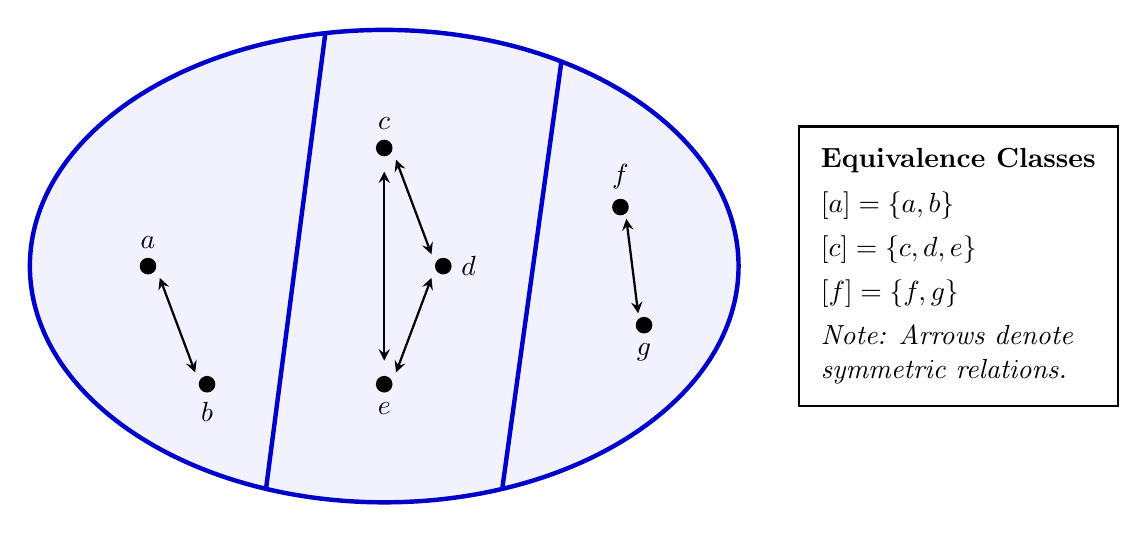
\begin{tikzpicture}[scale=1.5]
    % Background / Base shape
    \fill[blue!5!white] (0,0) ellipse (3 and 2);
    \draw[ultra thick, blue!80!black] (0,0) ellipse (3 and 2);
    
    % Partition lines
    \draw[ultra thick, blue!80!black] (-1, -1.88) -- (-0.5, 1.96);
    \draw[ultra thick, blue!80!black] (1, -1.88) -- (1.5, 1.73);
    
    % Nodes in Class 1
    \fill[black] (-2, 0) circle (2pt) node[above=3pt] {$a$};
    \fill[black] (-1.5, -1) circle (2pt) node[below=3pt] {$b$};
    \draw[thick, <->, >=stealth] (-1.9, -0.1) -- (-1.6, -0.9);
    
    % Nodes in Class 2
    \fill[black] (0, 1) circle (2pt) node[above=3pt] {$c$};
    \fill[black] (0.5, 0) circle (2pt) node[right=3pt] {$d$};
    \fill[black] (0, -1) circle (2pt) node[below=3pt] {$e$};
    \draw[thick, <->, >=stealth] (0.1, 0.9) -- (0.4, 0.1);
    \draw[thick, <->, >=stealth] (0.4, -0.1) -- (0.1, -0.9);
    \draw[thick, <->, >=stealth] (0, 0.8) -- (0, -0.8);
    
    % Nodes in Class 3
    \fill[black] (2, 0.5) circle (2pt) node[above=3pt] {$f$};
    \fill[black] (2.2, -0.5) circle (2pt) node[below=3pt] {$g$};
    \draw[thick, <->, >=stealth] (2.05, 0.4) -- (2.15, -0.4);
    
    % Legend using single node
    \node[align=left, anchor=west, draw, thick, fill=white, inner sep=8pt] at (3.5, 0) {
        \textbf{Equivalence Classes} \\[4pt]
        $[a] = \{a, b\}$ \\[4pt]
        $[c] = \{c, d, e\}$ \\[4pt]
        $[f] = \{f, g\}$ \\[4pt]
        \textit{Note: Arrows denote} \\
        \textit{symmetric relations.}
    };
\end{tikzpicture}
\end{center}

\subsection{Heuristics \& Pitfalls}
\begin{itemize}
    \item \textbf{Heuristic - The "Equality Check":} If you are unsure if a relation is an equivalence relation, ask yourself: "Does this relation act like an equals sign?" If it inherently measures a shared property (e.g., "has the same color as", "has the same remainder as"), it is almost certainly an equivalence relation.
    \item \textbf{Pitfall - The Empty Domain Trap:} A common fallacy is assuming that Symmetry + Transitivity $\implies$ Reflexivity. The false proof goes: $xRy \implies yRx$ (Sym). Then $xRy \land yRx \implies xRx$ (Trans). The flaw? This assumes there exists \textit{at least one} $y$ such that $xRy$. If $x$ is related to nothing, the premise fails, and $xRx$ is not guaranteed.
    \item \textbf{Pitfall - Overlapping Classes:} Beginners often accidentally define relations where an element can belong to two different classes (e.g., $a R b$ if they share a common factor $>1$). This fails transitivity and does not form a valid partition.
\end{itemize}

\newpage

\section{Conceptual Synthesis and The "Big Picture"}

\subsection{A) Thematic Connections}
The central theme of this topic is \textbf{Abstraction via Quotienting}. In mathematics, we often encounter sets that are too large or complex to study element-by-element. Equivalence relations allow us to "zoom out." By grouping elements that share a core property into a single equivalence class, we create a new, simplified set called a \textbf{Quotient Set} (denoted $A/R$). This theme unifies basic arithmetic (where we group infinite integers into finite modulo classes) with advanced geometry (where we group all congruent triangles into a single abstract "shape").

\subsection{B) Forward and Backward Links}
\begin{itemize}
    \item \textbf{Backward Links:} This topic builds directly on basic Set Theory (Cartesian products, subsets) and First-Order Logic. It provides a geometric and structural meaning to the abstract logical symbols $\forall$ and $\exists$.
    \item \textbf{Forward Links:} Equivalence relations are the absolute bedrock of Abstract Algebra and Topology. In algebra, they are used to construct Quotient Groups and Rings (e.g., constructing the real numbers from Cauchy sequences of rationals). In topology, they are used to construct complex spaces (like a torus or a Möbius strip) by "gluing" the edges of simple spaces (like a square) together—a process formally defined by an equivalence relation on the boundary points.
\end{itemize}

\section{Abstract Real-World Modeling (AI, ML, \& Quant Finance)}

\subsection{A) Concrete Scenarios}
\begin{enumerate}
    \item \textbf{State Space Reduction in Reinforcement Learning (AI):} In Markov Decision Processes (MDPs), the state space can be astronomically large (e.g., every possible pixel configuration on a screen). AI researchers use an equivalence relation called \textbf{Bisimulation} to group states that yield identical future reward distributions. The AI then learns a policy on the much smaller quotient MDP, drastically reducing computation time.
    \item \textbf{Asset Clustering in Quantitative Finance:} Quants often define equivalence relations (or relaxed tolerance relations) based on the correlation matrices of asset returns. Assets that are highly co-integrated are grouped into equivalence classes, allowing the portfolio optimizer to treat a basket of 500 stocks as a simplified set of 10 independent macroeconomic risk factors.
\end{enumerate}

\subsection{B) Model Problem Setup: MDP Bisimulation}
Let us rigorously model the AI scenario. Consider a Markov Decision Process defined by the tuple $\mathcal{M} = (S, A, P, R, \gamma)$, where $S$ is a finite state space, $A$ is a finite action space, $P(s'|s,a)$ is the transition probability, and $R(s,a)$ is the expected reward.

We define a relation $E \subseteq S \times S$. We say two states are bisimilar, denoted $s_1 E s_2$, if for all actions $a \in A$:
1. \textbf{Reward Equivalence:} $\displaystyle R(s_1, a) = R(s_2, a)$
2. \textbf{Transition Equivalence:} For every equivalence class $C \in S/E$, the probability of transitioning into $C$ is identical:
   \[ \displaystyle \sum_{s' \in C} P(s' | s_1, a) = \sum_{s' \in C} P(s' | s_2, a) \]

\textbf{Theoretical Objective:} To prove that $E$ is an equivalence relation, one must show it is reflexive, symmetric, and transitive. Once proven, we construct the \textbf{Quotient MDP} $\mathcal{M}_E = (S/E, A, P_E, R_E, \gamma)$. The optimal value function $V^*$ computed on $\mathcal{M}_E$ is mathematically guaranteed to lift back to the original space $S$ without any loss of optimality, effectively solving the "Curse of Dimensionality" for this specific environment.

\newpage

\section{Common Variations and Untested Concepts}

\subsection{Well-Defined Operations on Quotient Sets}
A critical concept not explicitly tested in the provided homework is proving that an algebraic operation is \textbf{well-defined} on a set of equivalence classes. When we define addition on equivalence classes, say $[a] \oplus [b] = [a+b]$, we must prove that the choice of representatives $a$ and $b$ does not change the result.

\textbf{Example Theorem:} Let $R$ be the modulo $n$ equivalence relation on $\Z$ ($a R b \iff n | (a-b)$). Prove that addition on $\Z/n\Z$ defined by $[a] \oplus [b] = [a+b]$ is well-defined.

\textbf{Rigorous Proof:}
1. To show the operation is well-defined, we must show that if we pick different representatives for the classes, the sum remains in the same resulting class.
2. Let $[a] = [a']$ and $[b] = [b']$. This means $a R a'$ and $b R b'$.
3. By definition, $a - a' = nk_1$ and $b - b' = nk_2$ for some $k_1, k_2 \in \Z$.
4. We must show that $[a+b] = [a'+b']$, which requires proving $(a+b) R (a'+b')$.
5. Consider the difference: $(a+b) - (a'+b') = (a - a') + (b - b')$.
6. Substituting our equations from step 3: $(a - a') + (b - b') = nk_1 + nk_2 = n(k_1 + k_2)$.
7. Since $k_1 + k_2 \in \Z$, we have $n | ((a+b) - (a'+b'))$.
8. Therefore, $(a+b) R (a'+b')$, meaning $[a+b] = [a'+b']$. The operation is well-defined. $\blacksquare$

\section{Advanced Diagnostic Testing: "Find the Flaw"}

Below are five proofs containing subtle logical or mathematical flaws. Your task as the grader is to identify the error. (The solutions are provided at the bottom).

\textbf{Problem 1:} Let $R$ be a relation on $A$. \textit{Proof that Symmetry and Transitivity imply Reflexivity:} Let $x \in A$. Choose a $y \in A$ such that $x R y$. By symmetry, $y R x$. By transitivity, since $x R y$ and $y R x$, we conclude $x R x$. Thus, $R$ is reflexive.

\textbf{Problem 2:} Let $R$ be defined on $\R$ by $x R y$ if $|x - y| \le 1$. \textit{Proof of Equivalence:} Reflexive: $|x - x| = 0 \le 1$. Symmetric: $|x - y| \le 1 \implies |y - x| \le 1$. Transitive: If $|x - y| \le 1$ and $|y - z| \le 1$, then $x, y, z$ are all close to each other, so $x R z$. Thus, $R$ is an equivalence relation.

\textbf{Problem 3:} Let $R$ be defined on $\Z$ by $a R b$ if $ab \ge 0$. \textit{Proof of Transitivity:} Assume $a R b$ and $b R c$. Then $ab \ge 0$ and $bc \ge 0$. Multiplying these inequalities gives $ab^2c \ge 0$. Since $b^2 \ge 0$, we can divide by $b^2$ to get $ac \ge 0$. Thus $a R c$.

\textbf{Problem 4:} Let $A = \{1, 2, 3\}$. We define a partition $P = \{\{1, 2\}, \{2, 3\}\}$. By the Partition Theorem, this defines an equivalence relation where $1 R 2$ and $2 R 3$.

\textbf{Problem 5:} Let $R$ be an equivalence relation on $A$. \textit{Proof that $[a] \cap [b] = \emptyset \implies a \neq b$:} Assume $[a] \cap [b] = \emptyset$. If $a = b$, then $[a] = [b]$, so $[a] \cap [b] = [a]$. Since equivalence classes are non-empty, $[a] \neq \emptyset$, contradicting the premise. Thus $a \neq b$. (Wait, is there a flaw here?)

\vspace{1em}
\hrule
\vspace{1em}
\textbf{Solution Key (The Flaws):}
\begin{itemize}
    \item \textbf{Flaw 1:} The proof assumes "Choose a $y \in A$ such that $x R y$." This assumes $x$ is related to \textit{something}. If $x$ is an isolated element related to nothing, the premise fails, and reflexivity cannot be established.
    \item \textbf{Flaw 2:} The transitivity proof uses vague language ("close to each other") instead of rigorous math. It is mathematically false: let $x=0, y=1, z=2$. $|0-1| \le 1$ and $|1-2| \le 1$, but $|0-2| = 2 \not\le 1$.
    \item \textbf{Flaw 3:} Division by zero. The proof divides by $b^2$. If $b = 0$, this division is undefined. Indeed, the relation fails transitivity at 0: $-1 R 0$ (since $-1 \cdot 0 = 0 \ge 0$) and $0 R 1$ (since $0 \cdot 1 = 0 \ge 0$), but $-1 \not R 1$ (since $-1 \cdot 1 = -1 < 0$).
    \item \textbf{Flaw 4:} The set $P$ is not a valid partition. By definition, the subsets in a partition must be \textit{pairwise disjoint}. $\{1, 2\} \cap \{2, 3\} = \{2\} \neq \emptyset$.
    \item \textbf{Flaw 5:} Trick question! There is no logical flaw in this proof. It is a perfectly valid proof by contrapositive/contradiction.
\end{itemize}

\end{document}